\section{实验过程记录}

\subsection{datapath的设计与仿真}
\begin{enumerate}
    \item datapath主要由pc,adder,alu,regfile等模块构成,均已完成或以提供,仅需要添加mux将各个端口连接即可
    \item controller模块已在实验二实现,将各个控制信号输入datapath,为mux,regfile提供控制信号
    \item inst\_ram,data\_ram直接调用ip核,由datapath输入pc,dataadr和writedata后,将readdata和inst输入datapath
    \item 在datapath内部,根据单周期的完整通路图,一一连接add、and、sub、or、slt、beq、j、lw、sw、addi等指令的数据通路即可
    \item 采用提供的testbench.v,把需要观察的信号从左侧添加到波形图中,然后重新进行仿真
    \item 调试完后无误则会执行最后一条sw指令,将\$2的7存到数据存储器的[84],并在控制台得到'Simulation succeeded'
\end{enumerate}


\subsection{问题1:inst比pc信号延迟}
\textbf{问题描述:}仿真后发现inst比pc慢了两个周期

\textbf{解决方案:}了解ip后发现选中Primitives Output Register会增加一个寄存器导致延时,但删除后还是延时了一个周期,推测pc的时钟比指令内存和数据内存的时钟慢得多,将原来的posedge clk改为negedge clk后变为正常
\begin{figure}[htbp]
    \centering
    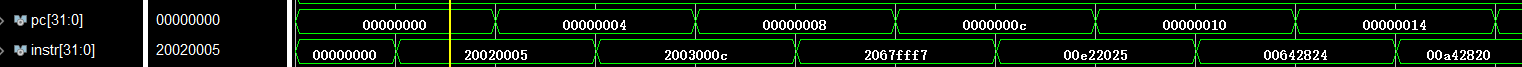
\includegraphics[width=0.9\textwidth]{q1.png}
    \label{图1}
\end{figure}

\subsection{问题2:数据读出异常}
\textbf{问题描述:}对指令的译码没有问题,但读不出RD的数据
\begin{figure}[htbp]
    \centering
    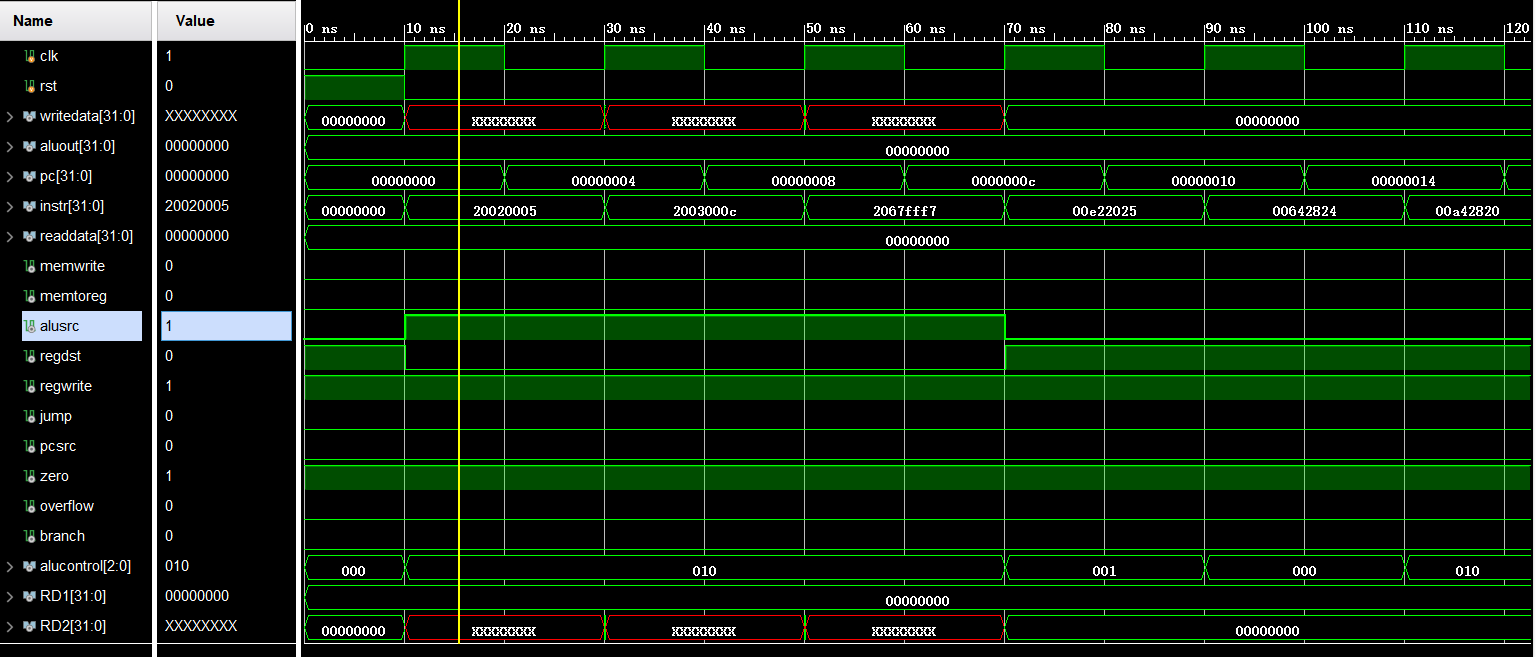
\includegraphics[width=0.9\textwidth]{q2.png}
    \label{图2}
\end{figure}

\textbf{解决方案:}发现datapath中一些名称过于相似混淆,如regwrite和writereg,或者将写入dataram的值和写入regfile的值搞混淆。另外源代码添加了过多无必要导线导致冗杂不方便阅读,删除后结果如下
\begin{figure}[htbp]
    \centering
    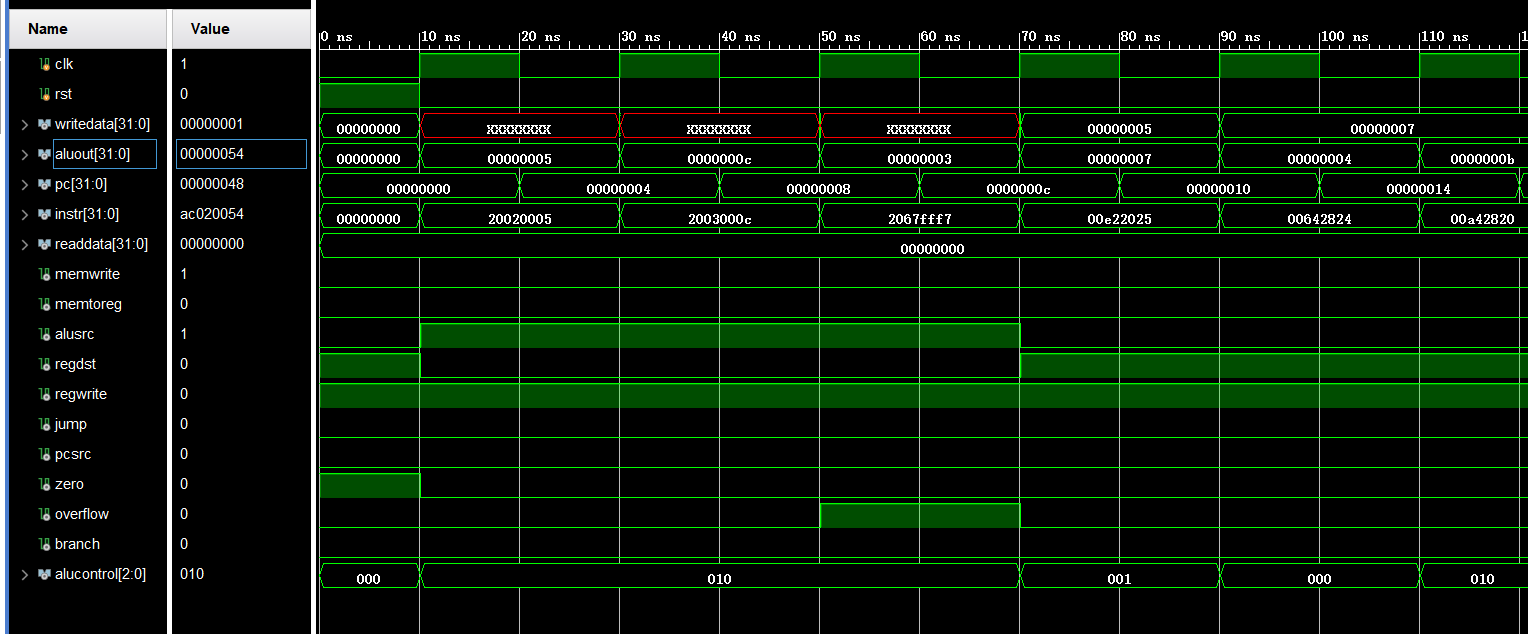
\includegraphics[width=0.9\textwidth]{q22.png}
    \label{图3}
\end{figure}

\subsection{问题3:beq指令无法跳转}
\textbf{问题描述:}branch信号有效却无法跳转

\textbf{解决方案:}为了解情况,将所有与pc有关信号加入wave中,发现pc,branch并没有在pc4的基础上加偏移,发现是sl2失效的原因,具体原因是sl2中的拼接位跳过了第一位,修改后正常
\begin{figure}[htbp]
    \centering
    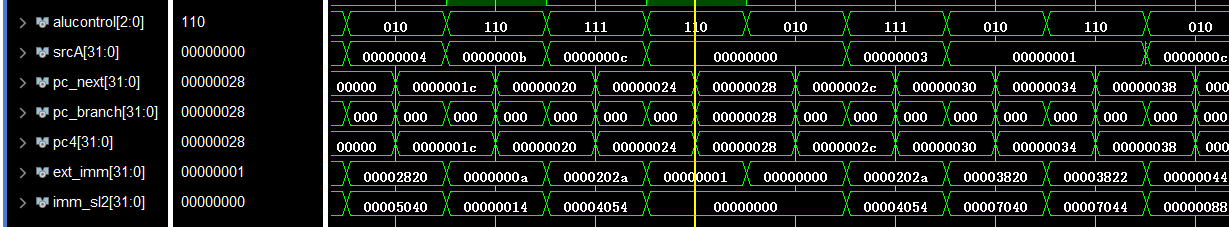
\includegraphics[width=0.9\textwidth]{q3.png}
    \label{图4}
\end{figure}
